\documentclass[8pt]{extarticle}
\usepackage[T1]{fontenc}
\usepackage[utf8]{inputenc}
\usepackage{lmodern}
\usepackage{ngerman}
\usepackage{listings}
\usepackage[letterpaper, margin=1.5cm]{geometry}
\usepackage{parskip}
\usepackage{titlesec}
\usepackage{color}
\usepackage{graphicx}
\usepackage{wrapfig}

\definecolor{grey}{rgb}{0.8, 0.8, 0.8}
\definecolor{darkblue}{rgb}{0.0, 0.18, 0.39}
\titleformat*{\section}{\small\bfseries\color{darkblue}}
\titlespacing{\section}{0pt}{\parskip}{-\parskip}
\graphicspath{ {../images/} } 

\lstset{frame=tb,
  aboveskip=1mm,
  belowskip=1mm,
  showstringspaces=false,
  columns=flexible,
  basicstyle={\small\ttfamily\color{darkblue}},
  breaklines=true,
  breakatwhitespace=true,
  rulecolor=\color{grey}
}
\renewcommand{\familydefault}{\sfdefault}
\pagestyle{empty}


\title{Instruction}
\author{Marie Lohbeck}

\begin{document}

\section*{Running PicDat}
Genaral usage: 
\begin{lstlisting}
picdat [--help] [--sortbyname] [--inputfile "input"] [--outputdir "output"] [--debug "level"]
\end{lstlisting}

You can run PicDat without any parameters. After you startet it, it'll ask you for some PerfStats. You can enter the path to a single file like output.data or to a whole folder with output.data files inside or to a zip folder. Additionally, PicDat will ask you to enter a directory for its results. Be aware, that content might get overwritten if this directory is not empty! After this, PicDat will start working. 

This is how the command line output could look like:
\begin{lstlisting}
python picdat.py
Please enter a path to some PerfStat output (folder or zipfolder or .data file, default is ./output.data):
</path/to/perfstat.out>
Please select a destination directory for the results (Default is ./results):
</path/to/output>
2017-09-28 15:57:02,988 INFO: inputfile: </path/to/perfstat.out>, outputdir: </path/to/output>
2017-09-28 15:57:02,989 INFO: Did not find a console.log file to extract perfstat's cluster and node name.
2017-09-28 15:57:02,989 INFO: Prepare directory...
2017-09-28 15:57:03,080 INFO: Read data...
2017-09-28 15:57:08,294 INFO: Planned number of iterations was executed correctly.
2017-09-28 15:57:08,297 INFO: Create csv tables...
2017-09-28 15:57:08,319 INFO: Wrote chart values into /path/to/output/tables/aggregate_total_transfers_chart_values.csv
2017-09-28 15:57:08,320 INFO: Wrote chart values into /path/to/output/tables/processor_processor_busy_chart_values.csv
2017-09-28 15:57:08,353 INFO: Wrote chart values into /path/to/output/tables/volume_total_ops_chart_values.csv
2017-09-28 15:57:08,354 INFO: Wrote chart values into /path/to/output/tables/volume_avg_latency_chart_values.csv
2017-09-28 15:57:08,365 INFO: Wrote chart values into /path/to/output/tables/volume_read_data_chart_values.csv
2017-09-28 15:57:08,370 INFO: Wrote chart values into /path/to/output/tables/lun_total_ops_chart_values.csv
2017-09-28 15:57:08,370 INFO: Wrote chart values into /path/to/output/tables/lun_avg_latency_chart_values.csv
2017-09-28 15:57:08,371 INFO: Wrote chart values into /path/to/output/tables/lun_read_data_chart_values.csv
2017-09-28 15:57:08,371 INFO: Wrote chart values into /path/to/output/tables/lun_read_align_histo_chart_values.csv
2017-09-28 15:57:08,372 INFO: Wrote chart values into /path/to/output/tables/sysstat_x_1sec_percent_chart_values.csv
2017-09-28 15:57:08,373 INFO: Wrote chart values into /path/to/output/tables/sysstat_x_1sec_MBs_chart_values.csv
2017-09-28 15:57:08,374 INFO: Wrote chart values into /path/to/output/tables/sysstat_x_1sec_IOPS_chart_values.csv
2017-09-28 15:57:08,374 INFO: Wrote chart values into /path/to/output/tables/statit_disk_statistics_chart_values.csv
2017-09-28 15:57:08,374 INFO: Create html file...
2017-09-28 15:57:08,414 INFO: Generated html file at /path/to/output/charts.html
2017-09-28 15:57:08,415 INFO: Done. You will find charts under: </path/to/output>
\end{lstlisting}

Alternatively, you can transmit Perfstat input and output directory as command line options. Therefore, use the options -\,-inputfile and -\,-outputdir or -i and -o respectively.

Another available command line option is the -\,-debug or -d flag. It specifies the filtering level for command line output. Pass it together with a string out of those: debug, info, warning, error, critical
Default is 'info'.

By default, PicDat sorts the different data series by relevance. This means, the graph with the highest sum of values will be displayed at the top of a chart's legend. If you rather wants them to be sorted alphanumeric, use the flag -\,-sortbyname or -s.

To get information about the usage, try option -\,-help or -h.
\bigskip

\section*{The output}
PicDat will search the .data files in your PerfStat input for some keywords, print the values into several csv tables and generates html files with charts. You'll find all output inside the directory you transmitted as outputdir. There, PicDat creates two subdirectories. One contains all csv tables, the other is called 'dygraphs' and contains files beeing necessary for visualization. For each .data file, PicDat found in your input, one charts.html will be generated.

\section*{Interactive charts}
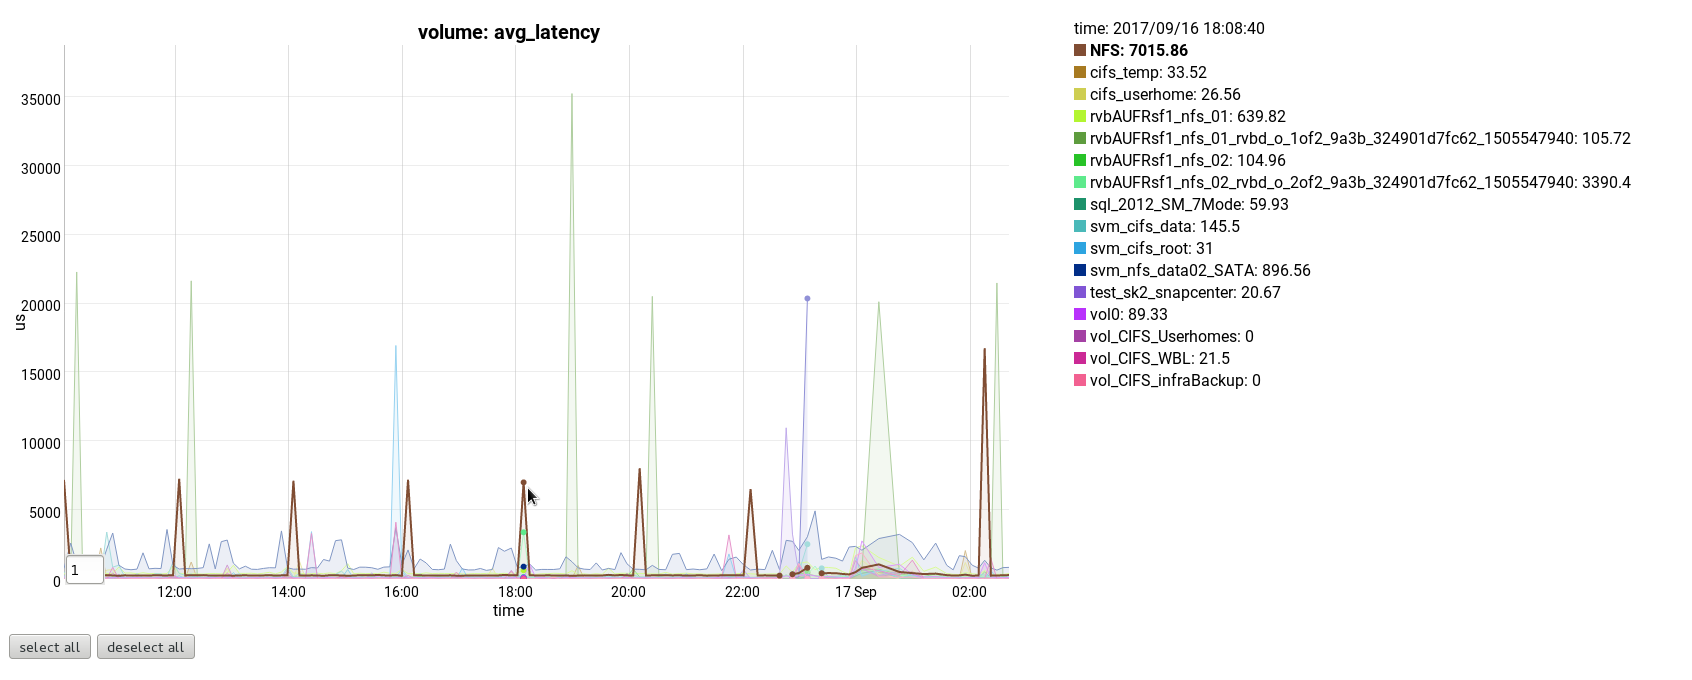
\includegraphics[scale=0.3]{PicDat_hightlight2}

The Job of PicDat is to pic and visualize some of the various information given in a PerfStat. The charts.html file contains several labeled charts offering some interaction. Mouse-over them to display the values in the legend. You'll notice as well, that the graph, your cursor is next, will be highlighted. The corresponding entry in the legend will be highlighted similtaneously.
To zoom inside the charts, just click and drag them in x or y direction. Once zoomed in, you can also change the displayed range by holding shift an click and drag again. To go back into original view, just double-click the chart.
\begin{wrapfigure}[10]{r}{0.6\textwidth}
    \centering
    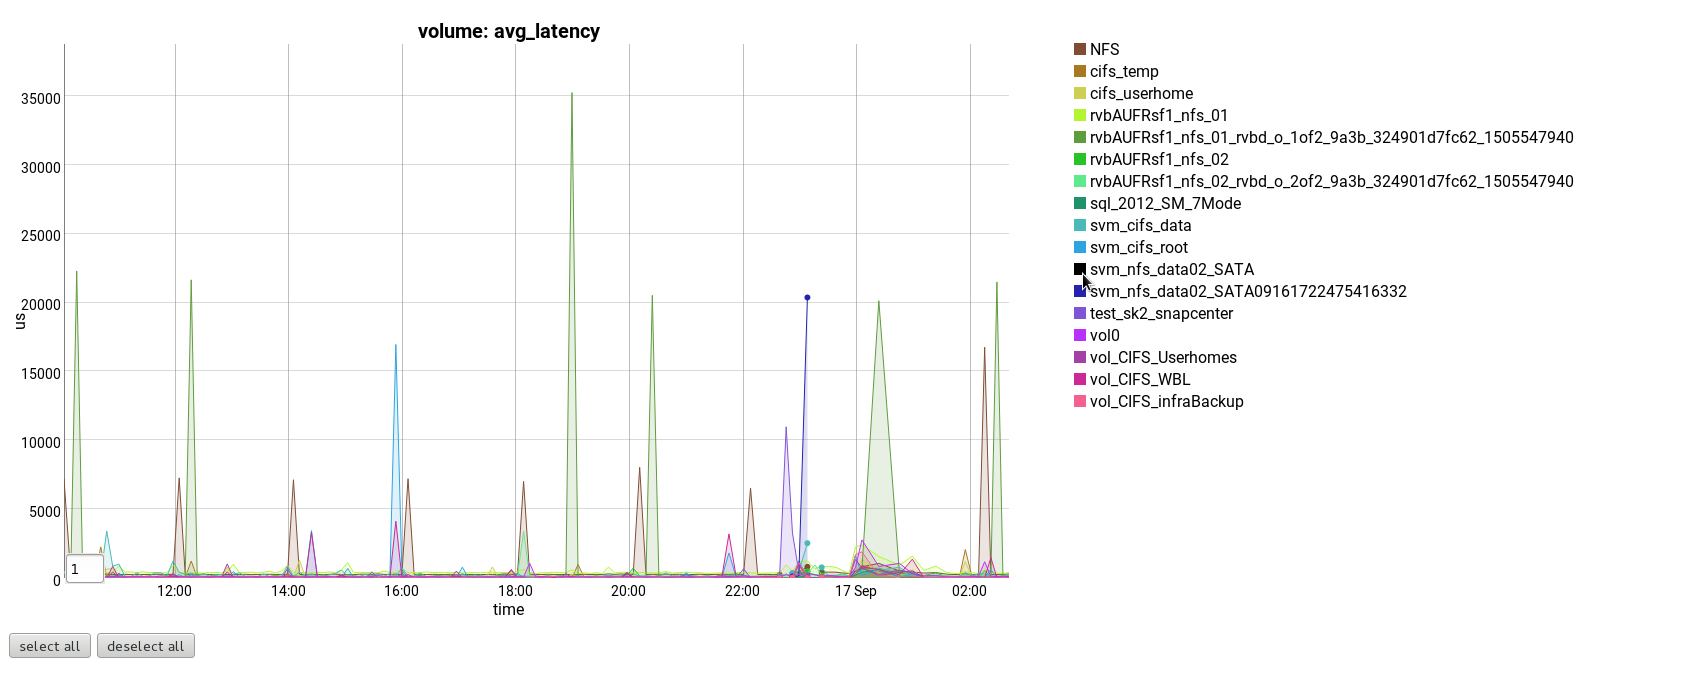
\includegraphics[scale=0.2]{PicDat_deselect}
\end{wrapfigure}
You might wish to take some graph lines out of view. Therefore, click one of the colored boxes inside the legend. It'll turn to black and the corresponding graph will disappear from sight. Click it again and the graph will come back. To select or deselect all lines at once, use the buttons beneath the chart.
Note, that disabled graphs disappear from the legend whereas your cursor is on the chart. Entries, belonging to graphs with a gap at the place your cursor recently is, will disappear as well. So don't be confused if the legend will bounce a bit as you move your mouse. 
\bigskip
\bigskip
\bigskip

If there are so many graphs in one chart that the legend can't display them all without a scroll bar, the legend will change to display only one value at once as soon as your mouse enters the chart.
 
If your values are very close and unsteady, you might get a better overview using a rolling average. Therefore, type a natural number into the small textfield appearing at the lower left corner of most charts. After hitting 'enter', the data will get averaged over this number of measuring points.
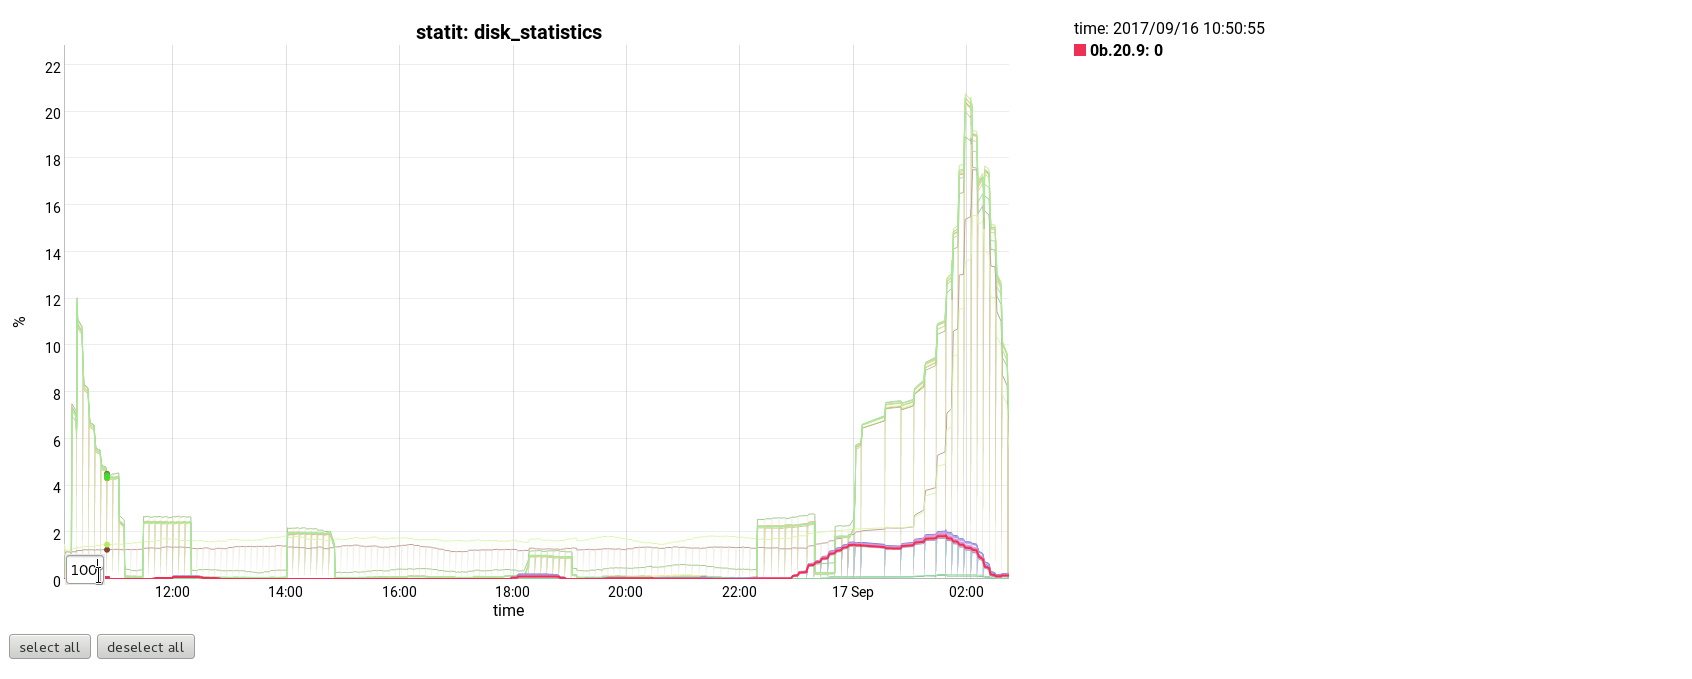
\includegraphics[scale=0.3]{PicDat_roller}
\bigskip

\section*{Can't see any graphs?}
If you are running the charts.html from your file system, the Browsers Chrome and Internet Explorer/Edge are blocking external files for security reasons. So, the dygraph.js can't be loaded. To avoid this, use Firefox instead, use a local web server or try to change security settings.
If this is not the problem, make sure that dygraphs is available at all. A folder called 'dygraphs', containing the dygraph.js and dygraph.css, must be in the same location as your charts.html file.

\end{document}
